\documentclass[xcolor=pdftex,dvipsnames,table,aspectratio=169]{beamer}
%\documentclass[xcolor=pdftex,dvipsnames,table,handout,aspectratio=169]{beamer}

%\setbeameroption{show notes}

\usepackage{bm,graphicx,multirow,amsmath,tikz} %fancybox,
\usepackage{color}%,textpos}
\usepackage[round]{natbib}
\usepackage[normalem]{ulem}
\usepackage{hyperref}
\usepackage{lastpage}
\usepackage{array}
\usepackage{color}
\usepackage{framed}
\usepackage{hyperref}

% Define Western colours
\definecolor{western}{rgb}{.306,.152,.524}
\definecolor{westerngray}{rgb}{.512,.508,.524}

%% Define BEAMER colours
\setbeamercolor{frametitle}{bg=western,fg=white}
\setbeamercolor{framesubtitle}{bg=western,fg=black}
\setbeamercolor{title}{fg=white,bg=western}
\setbeamercolor{author}{fg=white,bg=western}
\setbeamercolor{institute}{fg=white,bg=western}
\setbeamercolor{date}{fg=white,bg=western}

%% Set BEAMER fonts
\setbeamerfont{title}{shape=\bf}
\setbeamerfont{frametitle}{shape=\sc,size=\Large}
\setbeamerfont{framesubtitle}{shape=\sc,size=\Large}
\setbeamerfont{footline}{shape=\sc}

%% Define BEAMER toc
\setbeamercolor{section in toc}{fg=western}
\setbeamercolor{subsection in toc}{fg=westerngray}
\setbeamertemplate{sections/subsections in toc}[ball]

%% Define BEAMER background
\setbeamercolor{background canvas}{bg=white}

%% Define BEAMER footer
\setbeamertemplate{navigation symbols}{}
\setbeamercolor{footline}{fg=white,bg=western}
\setbeamertemplate{footline}{%
  \begin{beamercolorbox}[wd=\paperwidth]{footline}
    \vskip5pt

    \raisebox{.05in}{
      \scriptsize{\bf \insertshorttitle}
    }
    \hfill
    \raisebox{.05in}{
      \scriptsize{\bf \insertframenumber/\inserttotalframenumber} 
    }
    \hspace{5pt}

    \vskip5pt
  \end{beamercolorbox}
}

%% Define BLOCK environment
\setbeamercolor{block title}{fg=western}
\setbeamerfont{block title}{series=\bfseries}

%% Define ENUMERATE and ITEMIZE environements
\setbeamertemplate{itemize item}[ball]
\setbeamertemplate{enumerate item}[ball]
\setbeamercolor{item projected}{bg=western}

%% Define BEAMER toc
\setbeamercolor{sections/subsections in toc}{fg=blue!75}
\setbeamertemplate{sections/subsections in toc}[ball]

% %% Define SECTION openings
% \AtBeginSection[]{
%   \begin{frame}{\insertshorttitle}
%     \tableofcontents[currentsection,subsectionstyle=hide/hide/hide]
    
%   \end{frame}
% }

%% Define BEAMER frametitle
\addtobeamertemplate{frametitle}{
   \let\insertframetitle\insertsectionhead}{}
\addtobeamertemplate{frametitle}{
   \let\insertframesubtitle\insertsubsectionhead}{}


\makeatletter
  \CheckCommand*\beamer@checkframetitle{\@ifnextchar\bgroup\beamer@inlineframetitle{}}
  \renewcommand*\beamer@checkframetitle{\global\let\beamer@frametitle\relax\@ifnextchar\bgroup\beamer@inlineframetitle{}}
\makeatother

% Define counters for example and exercise
\newcounter{example}
\newcounter{exercise}

% Define example and exercise commands
\renewcommand{\example}
{\stepcounter{example}Example \lecturenum.\arabic{example}}
\newcommand{\examplectd}
{Example \lecturenum.\arabic{example}\ ctd}
\newcommand{\exercise}
{\stepcounter{exercise}Exercise \lecturenum.\arabic{exercise}}
\newcommand{\exercisectd}
{Exercise \lecturenum.\arabic{exercise}\ ctd}

\newcommand{\lecturenum}{21}

\title[SS2857]{Probability and Statistics I}
\subtitle{\lecturenum.~Expected Values, Covariance, Correlation}

\date{}

%% Add logo
% \titlegraphic{\includegraphics[height=2cm]{../uwo_logo_reversed}}

%% Initialize R


\begin{document}

{
\setbeamertemplate{footline}{}
\setbeamercolor{background canvas}{bg=western}

\begin{frame}
  \addtocounter{framenumber}{-1}

  \maketitle
\end{frame}
}

\begin{frame}
  \frametitle{\invisible{Hello}}
  
  \begin{center}
    \Large{\textbf{5.2 Expected Values, Covariance, and Correlation}}


  \end{center}
  
\end{frame}

\section{Expectations, Covariance, and Correlation}

\begin{frame}
  \frametitle{\invisible{Hello}}
  
  \begin{center}
    \Large{\textbf{5.2.1 Expected Values}}
  \end{center}
  
\end{frame}


\begin{frame}
  \begin{block}{Expected Values for Jointly Distributed RVs}
    Suppose that $X$ and $Y$ are jointly distributed discrete random variables with joint pmf $p(x,y)$. The expected value of any function of $X$ and $Y$, $h(X,y)$, is
    \[
      E[h(X,Y)]=
          \sum_{x}\sum_{y}h(x,y)p(x,y)
    \]
  \end{block}
\end{frame}

\begin{frame}
  \begin{block}{Expected Values for Jointly Distributed RVs}
    Suppose that $X$ and $Y$ are jointly distributed continuous random variables with pdf $f(x,y)$. The expected value of any function of $X$ and $Y$, $h(X,y)$, is
    \[
      E[h(X,Y)]=\int_{-\infty}^\infty \int_{-\infty}^\infty h(x,y) f(x,y)~dxdy 
    \]
  \end{block}
\end{frame}

\begin{frame}<handout:0>
  \begin{block}{Example 21.1 ctd}
    The simplest possible joint distribution is that for two Bernoulli random variables. Suppose that $X$ and $Y$ take the values $0$ and $1$ according to the following joint pmf:

    \begin{center}
      \begin{tabular}{c|cccc}
        $x$ & \multicolumn{2}{c}{0} & \multicolumn{2}{c}{1}\\
        $y$ & 0 & 1 & 0 & 1\\
        \hline
        $p(x,y)$ & $p_{00}$ & $p_{01}$ & $p_{10}$ & $p_{11}$.
      \end{tabular}
    \end{center}

    \begin{enumerate}[a)]
    \item What is the expected value of $XY$?
    \end{enumerate}
    
  \end{block}
\end{frame}

\begin{frame}
  \frametitle{\invisible{Hello}}
  
  \begin{center}
    \Large{\textbf{5.2.2 Covariance and Correlation}}
  \end{center}
  
\end{frame}


\begin{frame}
  \begin{block}{Covariance}
    The covariance between two random variables $X$ and $Y$ is
    \begin{align*}
      \mbox{Cov}(X,Y)
      =E[(X-\mu_x)(Y-\mu_Y)]\\
    \end{align*}
  \end{block}
\end{frame}

\begin{frame}
  \begin{block}{Covariance}
  
      The covariance between two discrete random variables $X$ and $Y$ is
    \begin{align*}
      \mbox{Cov}(X,Y)
      &=E[(X-\mu_x)(Y-\mu_Y)]\\
      &=\sum_{x}\sum_{y}h(x,y)p(x,y).
    \end{align*}
    
    The covariance between two continuous random variables $X$ and $Y$ is
    \begin{align*}
      \mbox{Cov}(X,Y)
      &=E[(X-\mu_x)(Y-\mu_Y)]\\
      &=\int_{-\infty}^\infty \int_{-\infty}^\infty h(x,y) f(x,y)~dxdy.
    \end{align*}

  \end{block}
\end{frame}

\begin{frame}
  \begin{block}{Shortcut Formula for Covariances}
    
    The covariance of any two random variables $X$ and $Y$ is
    \[
      \mbox{Cov}(X,Y)=E[(X-E(X))(Y-E(Y))].
    \]
    
    \bigskip
    
    It is often more efficient to use the shortcut formula
    \[
      \mbox{Cov}(X,Y)=E(XY)-E(X)E(Y). 
    \]
    
  \end{block}
\end{frame}

\begin{frame}
  \begin{block}{Correlation}
    The correlation (coefficient) of $X$ and $Y$ is
    \[
      \mbox{Corr}(X,Y)=\rho(X,Y)=\frac{\mbox{Cov}(X,Y)}{\sigma_X\sigma_Y}.
    \]
  \end{block}
\end{frame}

\begin{frame}
  \begin{block}{Correlation}
    Correlation measures the strength of the \textit{linear} relationship between two variables.

    \bigskip

    \begin{itemize}
    \item $\mbox{Corr}(X,Y)=-1$: $Y=aX + b$ for some $a<0$.
    \item $-1<\mbox{Corr}(X,Y)<0$: $Y\approx aX + b$ for some $a<0$.
    \item $\mbox{Corr}(X,Y)=0$: the best fitting line has slope 0.
    \item $0<\mbox{Corr}(X,Y)<1$: $Y\approx aX + b$ for some $a<>0$.
    \item $\mbox{Corr}(X,Y)=1$: $Y=aX + b$ for some $a>0$.
    \end{itemize}

  \end{block}
\end{frame}


 
\begin{frame}
  \begin{block}{\example}
  Each of the following plots represents the joint pmf of two random variables, $X$ and $Y$. The points, $(x,y)$ represent the possible values of $(X,Y)$. The distribution places equal probability, $1/6$, at each point.

    \begin{center}
      \begin{tabular}{cccc}
        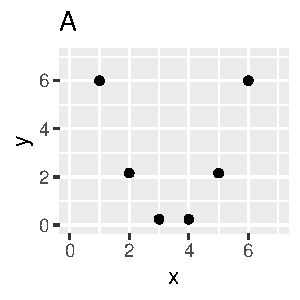
\includegraphics[height=.35\textheight]{figure/exercise-26-2-4} &
        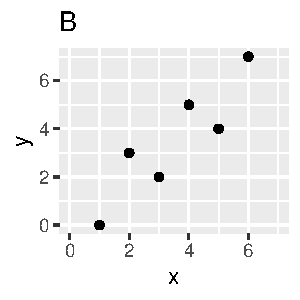
\includegraphics[height=.35\textheight]{figure/exercise-26-2-2} &
        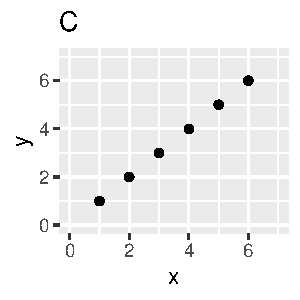
\includegraphics[height=.35\textheight]{figure/exercise-26-2-1} &
        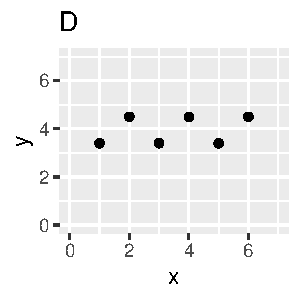
\includegraphics[height=.35\textheight]{figure/exercise-26-2-3} \\
      \end{tabular}
    \end{center}
    Order the plots according to their correlation.
    
  \end{block}
\end{frame}



\begin{frame}<handout:0>
  \begin{block}{\examplectd}
 Each of the following plots represents the joint pmf of two random variables, $X$ and $Y$. The points, $(x,y)$ represent the possible values of $(X,Y)$. The distribution places equal probability, $1/6$, at each point.

    \begin{center}
      \begin{tabular}{cccc}
        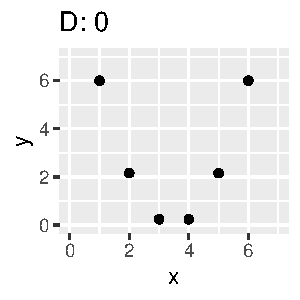
\includegraphics[height=.35\textheight]{figure/exercise-26-2b-4} &
        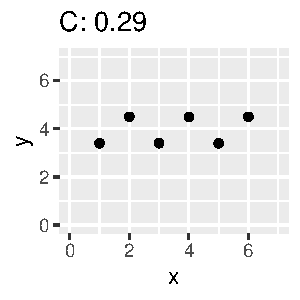
\includegraphics[height=.35\textheight]{figure/exercise-26-2b-3} &
        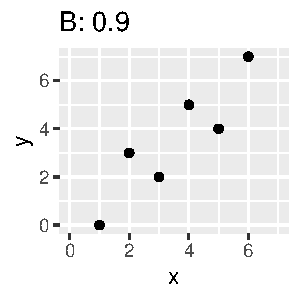
\includegraphics[height=.35\textheight]{figure/exercise-26-2b-2} &
        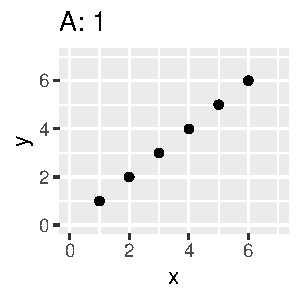
\includegraphics[height=.35\textheight]{figure/exercise-26-2b-1} 
      \end{tabular}
    \end{center}
    Order the plots according to their correlation.
    
  \end{block}
\end{frame}

\begin{frame}<handout:0>
  \begin{block}{Example 21.1 ctd}
    The simplest possible joint distribution is that for two Bernoulli random variables. Suppose that $X$ and $Y$ take the values $0$ and $1$ according to the following joint pmf:

    \begin{center}
      \begin{tabular}{c|cccc}
        $x$ & \multicolumn{2}{c}{0} & \multicolumn{2}{c}{1}\\
        $y$ & 0 & 1 & 0 & 1\\
        \hline
        $p(x,y)$ & $p_{00}$ & $p_{01}$ & $p_{10}$ & $p_{11}$.
      \end{tabular}
    \end{center}
    \begin{enumerate}
    \item What is the expected value of $XY$?
    \item What are the covariance and correlation of $X$ and $Y$?
    \end{enumerate}
  \end{block}
\end{frame}

\begin{frame}
  \frametitle{\invisible{Hello}}
  
  \begin{center}
    \Large{\textbf{5.2.3 Sums of Random Variables}}
  \end{center}
  
\end{frame}

\begin{frame}
  \begin{block}{Sums of Random Variables}
    Let $X_1,X_2,\ldots$ be any sequence of random variables and $c_1,c_2,\ldots$ be any sequence of constants. Then
    \[
      E\left[\sum c_kX_k\right]=\sum c_k E(X_k).
    \]
    
    \bigskip 
    
    The sum may either be finite or infinite.
    
    \bigskip
    
    In the case of two random variables
    \[
      E(aX + bY)=aE(X) + bE(Y). 
    \]
    
  \end{block}
\end{frame}

\begin{frame}
  \begin{block}{Variance of a Sum of Random Variables}
    Let $X$ and $Y$ be any two random variables and $a,b \in \Re$. Then
    \[
    \mbox{Var}(aX + bY)=a^2 \mbox{Var}(X) + 2ab\mbox{Cov}(X,Y) + b^2\mbox{Var}(Y). 
    \]
    
    \bigskip
    
    If $X$ and $Y$ are independent then $\mbox{Cov}(X,Y)=0$\footnote{The reverse is \textbf{not} true in general.} In this case
    \[
    \mbox{Var}(aX + bY)=a^2 \mbox{Var}(X) + b^2\mbox{Var}(Y).
    \]
  \end{block}
\end{frame}

\begin{frame}<handout:0>
  \begin{block}{Example 21.1 ctd}
    The simplest possible joint distribution is that for two Bernoulli random variables. Suppose that $X$ and $Y$ take the values $0$ and $1$ according to the following joint pmf:

    \begin{center}
      \begin{tabular}{c|cccc}
        $x$ & \multicolumn{2}{c}{0} & \multicolumn{2}{c}{1}\\
        $y$ & 0 & 1 & 0 & 1\\
        \hline
        $p(x,y)$ & $p_{00}$ & $p_{01}$ & $p_{10}$ & $p_{11}$.
      \end{tabular}
    \end{center}

    \begin{enumerate}
    \item What is the expected value of $XY$?
    \item What are the covariance and correlation of $X$ and $Y$?
    \item What are the mean and variance of $Z=2X + 4Y$?
    \end{enumerate}
  \end{block}
\end{frame}

\begin{frame}
  \frametitle{\invisible{Hello}}
  
  \begin{center}
    \Large{\textbf{5.2.4 Products of \textit{Independent} Random Variables}}
  \end{center}
  
\end{frame}

\begin{frame}
  \begin{block}{Products of Independent Random Variables}
    Let $X_1,X_2,\ldots$ be any set of independent random variables. Then 
    \[
    E\left[\prod X_k \right]=\prod E(X_k).
    \]
    
    \bigskip
    
    In the case of two independent random variables
    \[
      E(XY)=E(X)E(Y). 
    \]
    
  \end{block}
\end{frame}

\begin{frame}<handout:0>
  \begin{block}{Example 21.1 ctd}
    The simplest possible joint distribution is that for two Bernoulli random variables. Suppose that $X$ and $Y$ take the values $0$ and $1$ according to the following joint pmf:

    \begin{center}
      \begin{tabular}{c|cccc}
        $x$ & \multicolumn{2}{c}{0} & \multicolumn{2}{c}{1}\\
        $y$ & 0 & 1 & 0 & 1\\
        \hline
        $p(x,y)$ & $p_{00}$ & $p_{01}$ & $p_{10}$ & $p_{11}$.
      \end{tabular}
    \end{center}

    \begin{enumerate}
    \item What is the expected value of $XY$?
    \item What are the covariance and correlation of $X$ and $Y$?
    \item What are the mean and variance of $Z=2X + 4Y$?
    \item Under what conditions are $X$ and $Y$ independent? What is are the mean $XY$ in this case?
    \end{enumerate}
  \end{block}
\end{frame}

\begin{frame}<handout:0>
  \begin{center}
    \Huge{\textbf{Questions?}}
  \end{center}
\end{frame}

\begin{frame}

\begin{block}{\exercise}
Consider rolling two fair, three-sided die. Let $S$ denote the sum of the values showing on the two die and $D$ the absolute value of the difference. E.g., if one die shows the value 1 and the second shows the value 2 then $S=3$ and $D=1$, regardless of which was thrown first.

\begin{enumerate}[a)]
\item Construct a table showing the joint pmf of $S$ and $D$. 
\item Compute the marginal pmf of both $S$ and $D$. 
\item Compute the expected value and variance of $S$ and $D$.
\item Compute the covariance and correlation of $S$ and $D$. 
\item Are $S$ and $D$ independent? Justify your answer.
\end{enumerate}

\end{block}
\end{frame}
\end{document}
